\chapter{Project management}
\section{SCRUM}
\subsection{The principle}
Project management is an essential element in guaranteeing the success of a project. For our project, we chose to adopt an approach based on agile methods, in particular the Scrum method. Agile methods are characterized by their flexibility, adaptability and iterative approach, making them particularly well suited to complex, evolving projects.\\
\\
The Scrum method is one of the most popular and widely used agile methods. Key Scrum practices include daily coordination meetings, during which each team member shares his or her progress, challenges and plans for the future. Sprint planning meetings are used to define the sprint objectives and select the features to be implemented. At the end of each sprint, a retrospective meeting is held to evaluate the previous sprint and identify improvements for future sprints.\\
\\
In our project, we implemented the method by organizing our team with specific roles: the Scrum Master and the development team.\\
\\
The Scrum Master is responsible for facilitating the Scrum process, removing obstacles and ensuring that the team follows Scrum principles and practices. He also ensures that the necessary meetings and interactions take place.\\
\\
The development team is responsible for completing project tasks and delivering functionality at the end of each iteration, called a "sprint". Sprints are short, intensive work cycles, generally lasting two to four weeks, during which the development team focuses on delivering the highest-priority features.\\
\\

\subsection{Adaptation for our project}
To adapt the Scrum method to our project, we made adjustments to meet our specific needs and constraints. The adaptations we made include:\\
\begin{enumerate}

\item \textbf{Sprint size and duration:} we started with one-week sprints accompanied by a weekly meeting. Then we adapted the duration of the sprints to the amount of work required.

\item \textbf{Team composition:} Ms Croitoru is our Scrum Master, and we make up the development team.
\item \textbf{Adapting meetings :} We have adjusted some Scrum rituals to better suit our needs. For example, during daily meetings, we have added a brief discussion of obstacles and specific problems encountered by the team, in order to resolve them more effectively.\\
\end{enumerate}
Using the Scrum method gave us a number of advantages, such as better visibility of project progress, rapid adaptation to changes and close collaboration between team members. Agile principles also fostered open and transparent communication, stimulating team commitment.\\

\begin{figure}[!h]
\centering
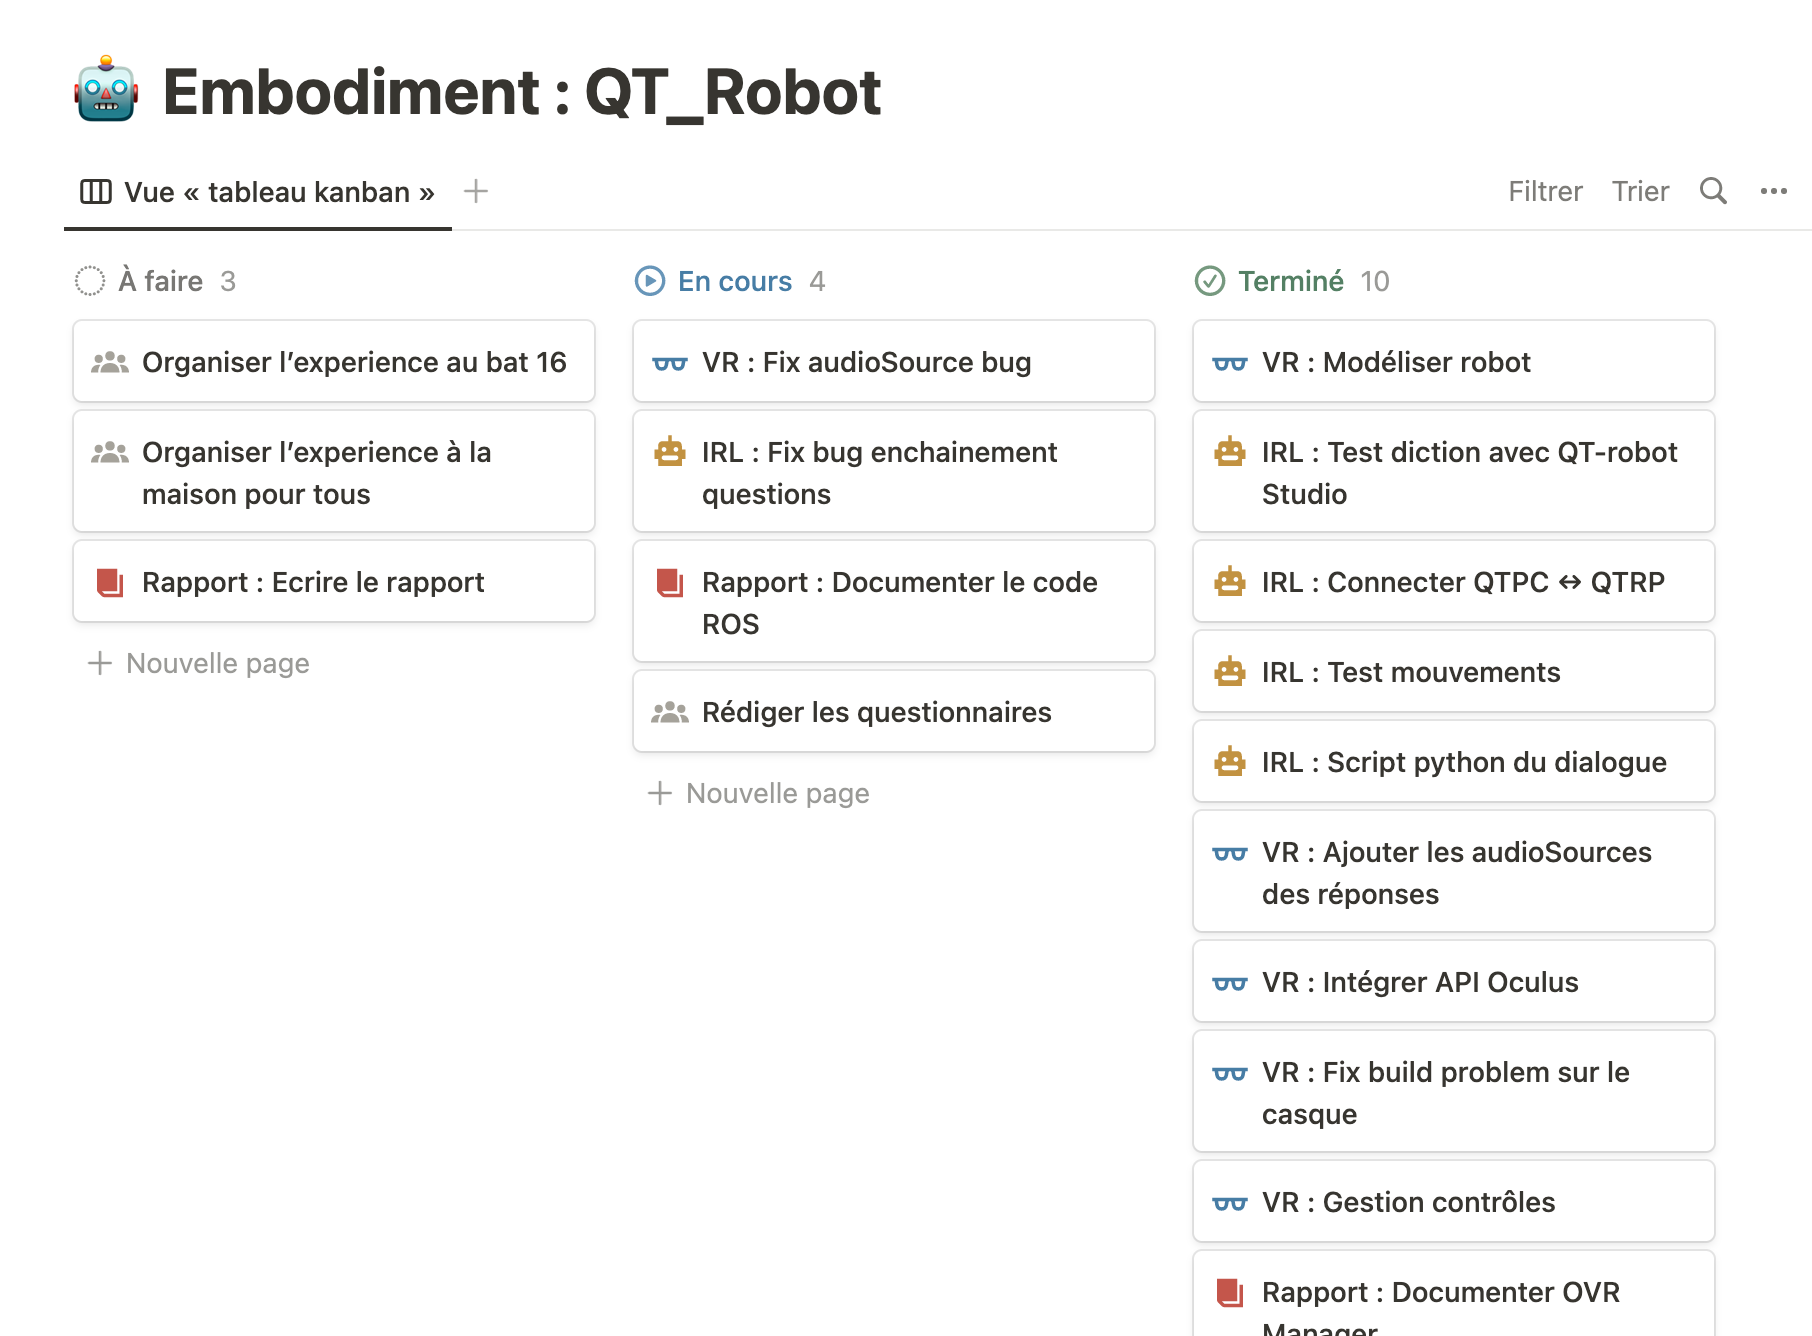
\includegraphics[height=10cm]{Figures/kanban.png}
\caption{Task kanban table - Notion}
\end{figure}

\newpage
\subsection{Distribution of tasks}
To optimize our efficiency, we chose to set up two-person mini-groups. This approach enabled us to take advantage of the complementary skills and knowledge of each team member, thus promoting greater productivity.
We thus set up two distinct groups, one dedicated to the development of the QTrobot and the other to virtual reality. Nevertheless, each person had the opportunity to work on both areas, which favored a thorough understanding of the project as a whole. \\
\\
Within each group, members worked in peer programming sessions. This method involves two developers working together on the same task, regularly exchanging ideas, solving problems together and ensuring the quality of the code produced. This enabled us to benefit from different points of view and find solutions more quickly.

\section{Tools used}
\subsection{Communication tools}
In addition to meetings with our supervisor at the IT building and at Lirmm, we used two essential communication tools: WhatsApp and Discord. These platforms played a key role in the coordination and collaboration between our team members.\\
\\
WhatsApp is an instant messaging application widely used around the world. We used it to facilitate fast, direct communication between the team and our project manager. WhatsApp's user-friendly interface and availability on smartphones make it a practical choice for instant communication.\\
\\
Discord, meanwhile, offers a host of features that foster online collaboration, such as chat rooms organized by category, voice channels for group calls and the ability to share files. We've used Discord for virtual meetings and group discussions, as well as for sharing important updates and resources. \\
\\
Using WhatsApp and Discord has greatly improved our efficiency and productivity as a team. These tools enabled seamless, instant and synchronized communication, promoting real-time collaboration. \\

\newpage
\subsection{Management tools}
We used two essential management tools to efficiently organize and manage our documents, information and tasks: Google Drive and Notion. We also used Overleaf to write the report in LaTeX.\\
\\
Google Drive is an online storage and file collaboration solution. We used it to create and share documents and photos. This platform enabled us to work simultaneously on the same files, promoting real-time collaboration. In particular, we used it to write and share roadmaps and meeting minutes, to keep a clear record of our progress. We also used the drive to share sound files, enabling us to implement voices for VR. \\
\\
Notion is a project management platform. We used it to organize our tasks, create checklists and track the progress of our various activities. The platform gave us an overview of all our tasks and deadlines, which helped us stay organized and meet our sprint deadlines. What's more, Notion allowed us to centralize all our important information in one place, facilitating sharing and collaboration between team members.\\